\documentclass[twoside]{article}
\usepackage[utf8]{inputenc}
\usepackage[ngerman]{babel}
\usepackage{libertine}
\usepackage[a4paper]{geometry}
\usepackage{parskip}
\usepackage{amsmath, amsthm, amssymb, commath, mathtools}
\usepackage{cancel}
\usepackage{physics}
\usepackage{nicefrac}
\usepackage{booktabs}
\usepackage{tabularx}
\usepackage{enumitem}
\usepackage{graphicx}
\usepackage{wrapfig}
\usepackage{caption}
\usepackage{float}
\usepackage{minted}
\usepackage{appendix}
\usepackage{icomma}
\usepackage{multirow}
\usepackage{multicol}
\usepackage{footmisc}
\usepackage[separate-uncertainty=true]{siunitx}
\sisetup{locale = DE}
\usepackage{xcolor}

\usepackage{csquotes}
\MakeOuterQuote{"}
\renewcommand{\ttdefault}{cmtt}

\usepackage{hyperref}
\usepackage{bookmark}
% https://tex.stackexchange.com/a/33701
\makeatletter
    \newcommand{\nonum}[0]{%
        \let\@oldseccntformat\@seccntformat %
        \renewcommand\@seccntformat[1]{}%
        }
    \newcommand{\resnum}[0]{\let\@seccntformat\@oldseccntformat}
\makeatother

\usepackage{chngcntr}
\counterwithin{figure}{section}

\newcommand{\versuch}[0]{STW}
\newcommand{\versuchLang}[0]{Stehende Wellen}

\hypersetup{
	pdftitle={P1 -- \versuch{} Auswertung},
	pdfauthor={Yudong Sun},
	bookmarksnumbered=true,
	bookmarksopen=true,
	bookmarksopenlevel=2,
	pdfstartview=Fit,
	pdfpagemode=UseOutlines,
	colorlinks=true,
	linkcolor=black,
	filecolor=magenta,      
	urlcolor=blue
}
\urlstyle{same}

\title{\versuch{} -- \versuchLang \\ Auswertung}
\author{Yudong Sun \\{\small in Zusammenarbeit mit David Giesegh und Joel Schönberger}\\\\ Gruppe F2}

\usepackage{fancyhdr}
\pagestyle{fancy}
\fancyhf{}
\fancyhead[RO]{Yudong Sun}
\fancyhead[LO]{Auswertung -- \versuch}
\fancyhead[LE]{Yudong Sun}
\fancyhead[RE]{Auswertung -- \versuch}
\cfoot{\thepage}

% Custom Defs
\newcommand*{\ra}[1]{\renewcommand{\arraystretch}{#1}}
\newcommand*{\maxi}[1]{\text{max}\left(#1\right)}
\newcommand*{\mini}[1]{\text{min}\left(#1\right)}
\newcommand*{\todo}[1]{\textcolor{red}{TODO: #1}}
\newcommand*{\iu}[1]{\textit{\underline{#1}}}
\newcommand*{\gnuplot}[0]{\texttt{gnuplot}}
\newcommand*{\captionbr}[0]{\\\rule{\textwidth}{0pt}\\\vspace{-\baselineskip}}
\newcommand*{\sigfig}[1]{\hspace{0.5cm}\text{(#1 sig. Zif.)}}
\newcommand*{\pbrace}[1]{\left(#1\right)}
\newcommand*{\sbrace}[1]{\left[#1\right]}
\newcommand*{\bDelta}[1]{\pbrace{\Delta #1}}
\newcommand*{\overbar}[1]{\overline{\raisebox{0pt}[1.2\height]{$#1$}}} % https://tex.stackexchange.com/a/87615

% \addto\captionsngerman{
%     \let\oldfigname\figurename
%     \renewcommand{\figurename}{[\oldfigname}
%     \let\oldthefig\thefigure
%     \renewcommand{\thefigure}{\oldthefig]}
% } % https://tex.stackexchange.com/a/17490
% https://tex.stackexchange.com/a/101624 new line in caption

% Gaußsche Fehler Erzeuger
\makeatletter
    \newcommand{\gausserror}[2]{% \gausserror{G}{faktoren}
        \sqrt{%
            \@tempswafalse
            \@for\factor:=#2
            \do{
                \if@tempswa+%
                \else%
                    \@tempswatrue%
                \fi%
                \left(\pdv{#1}{\factor}\Delta\factor\right)^2%
            }%
        }
    }
\makeatother
% https://tex.stackexchange.com/a/59912
% https://riptutorial.com/latex/example/28657/loops---repeating-things

% / Custom Defs

\begin{document}

\maketitle

% Einstellungen
\nonum
\numberwithin{equation}{section}
% / Einstellungen

\section{Teilversuch 1: "Gewichtsverlust" des Maxwellschen Rads}
    Das Maxwellsche-Rad hat während des Auf- und Abrollens (außer Umkehrpunkt) immer eine nach unten gerichtete Beschleunigung. Diese Beschleunigung wirkt in derselben Richtung wie die Erdbeschleunigung. Im Vergleich zum Ruhezustand zieht das Maxwellsche-Rad deswegen nicht so viel auf dem Faden. Das folgt aus der sichtbaren Beschleunigung während des Auf- und Abrollens und dem Newtonsche 3. Gesetz. Die gemessene Kraft ist folglich geringer und die Waage hebt sich ab. 

    Am tiefsten Punkt kehrt das Rad um. Das führt zu einer Impulsänderung in einem kurzen Zeitintervall von einem maximalen Impuls nach unten zu einem maximalen Impuls nach oben. Mit $F = \dv{p}{t}$ versteht man diese Impulsänderung als eine große Kraft, die auf den Faden zieht. Diese Kraft wurde als einen Zuck auf der Waage beobachtet. 

    Die Gewichtskraft und die Seilkraft wirken immer auf dem Rad. Da das Rad ab und aufrollt, sind diese zwei Kräfte nicht im Gleichgewicht und es gibt eine resultierende externe Kraft, die den Translationsimpuls des Rads ändert. Da die Seilkraft nicht am Schwerpunkt des Rads greift, gibt es auch ein Drehmoment bezüglich der Rotationsachse des Rads, die den Drehimpuls ändert. 

    Es gibt deshalb zu jedem Zeitpunkt eine externe Kraft bzw. Drehmoment auf dem Rad, und folglich ist das Rad kein Inertialsystem. Die Translation- und Drehimpuls bleiben dann auch nicht konstant. 
\section{Teilversuch 2: Bestimmung eines Reflexiongrades}
	Mit $A =$ die korrigierte maximale Amplitude und $B =$ die korrigierte minimale Amplitude ist das Reflexionsgrad $R$ und folglich dessen Fehler laut der Anleitung gegeben durch:
	\begin{align}
		R &= \pbrace{\frac{A+B}{A-B}}^2 \label{eqn:tv2-1} \\
		\Delta R &= \gausserror{R}{A,B}
	\end{align}
	Die partielle Ableitungen liefern jeweils:
	\begin{align}
		\pdv{R}{A} &= 2 \pbrace{\frac{A-B}{A+B}}\sbrace{\frac{\cancel{A}+B-\pbrace{\cancel{A}-B}}{\pbrace{A+B}^2}} = 2 \pbrace{\frac{A-B}{A+B}} \sbrace{\frac{2B}{\pbrace{A+B}^2}} \notag \\
		&= 4\cdot \frac{B\pbrace{A-B}}{\pbrace{A+B}^3} \\
		\pdv{R}{B} &= 2 \pbrace{\frac{A-B}{A+B}}\sbrace{\frac{-\pbrace{A+\cancel{B}}-\pbrace{A-\cancel{B}}}{\pbrace{A+B}^2}} = 2 \pbrace{\frac{A-B}{A+B}} \sbrace{\frac{-2A}{\pbrace{A+B}^2}} \notag \\
		&= -4\cdot \frac{A\pbrace{A-B}}{\pbrace{A+B}^3}
	\end{align}
	Da $\Delta A = \Delta B = \sqrt{2}\cdot\Delta S$, lässt der Fehler wie folgt schreiben:
	\begin{equation}
		\Delta R = 4\sqrt{2}\Delta S \frac{A-B}{\pbrace{A+B}^3}\sqrt{A^2+B^2} \label{eqn:tv2-2}
	\end{equation}
	wobei $\Delta S =$ der Fehler bei jeder Messung der Mikrofonspannung.

	Die korrigierte Minima und Maxima werden hier als Zwischenergebnisse behandelt. Darum werden keine Fehler explizit berechnet. Die ist aber durch $\sqrt{2}\Delta S$ gegeben.

	Der Mittelwert $\overbar{R}$ und dessen Fehler $\Delta R$ mittels der Methode der oberen und unteren Grenzen sind dann:
	\begin{align}
		\overbar{R} &= \frac{\sum_{i=1}^3 R_i}{3} \label{eqn:tv2-3} \\
		\Delta \overbar{R} &= \frac{\sum_{i=1}^3 \pbrace{\cancel{R_i} + \Delta R_i} - \sum_{i=1}^3 \pbrace{\cancel{R_i} - \Delta R_i}}{3 \times 2}  = \frac{\sum_{i=1}^3 \Delta R_i + \cancel{\sum_{i=1}^3 \Delta R_i}}{3 \times \cancel{2}} \notag \\
		&= \frac{\sum_{i=1}^3 \Delta R_i}{3} \label{eqn:tv2-4}
	\end{align}
	Da es nur beim zweiten Teilaufgabe der Auswertung zum Teilversuch 2 gefragt, dass man der Fehler $\Delta \overbar{R}$ mittels der Methode der oberen und unteren Grenzen berechnen soll, ist die Korrektur für $A$ und $B$ mittels Gauß'sche Fehlerfortpflanzung gerechnet. Außerdem ist auch schwerig, schnell zu bestimmen, wann $A$ bzw. $B$ jeweils maximal und minimal sein, um das maximales und minimales $R$ zu bekommen. 

	Mit Gleichungen \eqref{eqn:tv2-1}, \eqref{eqn:tv2-2}, \eqref{eqn:tv2-3} und \eqref{eqn:tv2-4}, darstellen wir die Ergebnisse als Tabelle. Die Rechnungen erfolgt genauer in einem Tabellenkalkulationsprogramm. Die Werte hier sind schon gerundet. 
	\begin{center}
		\begin{tabular}{lrrr r}
			\toprule
			Paar $i$ & \num{1} & \num{2} & \num{3} & \\
			\midrule
			Min $S_\text{min} / \si{\milli\volt}$ & \num{5.8} & \num{6.2} & \num{6.0} & \\
			Hintergr. $S_\text{min HG} / \si{\milli\volt}$ & \num{0.9} & \num{0.9} & \num{0.9} & \\
			Max $S_\text{max} / \si{\milli\volt}$ &\num{20.7} & \num{20.1} & \num{20.5} & \\
			Hintergr. $S_\text{max HG} / \si{\milli\volt}$ & \num{0.9} & \num{0.9} & \num{1.0} & \\
			\midrule
			$B / \si{\milli\volt}$ & \num{4.9} & \num{5.3} & \num{5.1} & \\
			$A / \si{\milli\volt}$ & \num{19.8} & \num{19.2} & \num{19.5} & \\
			$R$ & \num{0.364} & \num{0.322} & \num{0.343} & $\overbar{R} = \num{0.343}$ \\
			$\Delta R$ & \num{0.023} & \num{0.022} & \num{0.023} & $\Delta \overbar{R} = \num{0.023}$ \\
			\bottomrule
		\end{tabular}
	\end{center}
	Explizit geschrieben: $R = \num{0.343(23)}$. $R$ is einheitslos. 

	Als Funktion der Energie ist $R$ gegeben durch:
	\begin{equation}
		R = \frac{b^2}{a^2} = \frac{\text{Energie der reflektierten Welle}}{\text{Energie der Quellwelle}}
	\end{equation}
	Laut Energieerhaltungssatz kann die reflektierte Welle keine Energie mehr als die Quellwelle haben. Das heißt, dass $b < a$ bzw. $R \in \sbrace{0,1}$ sein muss. In diesem Fall liegt unser Wert von $R$ in diesem Intervall, was physikalischen Sinn ergibt.

	In unserem Versuch ist $\SI{34.3(23)}{\percent}$ der Energieflussdichte am offenen Rohrende reflektiert und $\SI{100}{\percent} - \SI{34.3(23)}{\percent} = \SI{65.7(23)}{\percent}$ transmittiert.
\newpage
\section{Teilversuch 3: Messung der Eigenfrequenzen einer Luftsäule}
	Fehler bei Messung bzw. Steuerung der Frequenz $\Delta f_n = \SI{1}{\hertz}$\\
	Fehler bei Messung der Mikrofonspannung $\Delta U_\text{eff} = \SI{0.1}{\milli\volt}$

	\begin{center}
		\begin{tabular}{l *{11}{r}}
			\toprule
			$n$ & \num{0} & \num{1} & \num{2} & \num{3} & \num{4} & \num{5} & \num{6} & \num{7} & \num{8} & \num{9} & \num{10} \\
			\midrule
			$f_n / \si{\hertz}$ & \num{168} & \num{502} & \num{837} & \num{1171} & \num{1510} & \num{1843} & \num{2188} & \num{2541} & \num{2876} & \num{3210} & \num{3554} \\
			$U_\text{eff} / \si{\milli\volt}$ & \num{3.36} & \num{22.10} & \num{57.7} & \num{31.07} & \num{21.70} & \num{22.48} & \num{22.93} & \num{24.80} & \num{13.20} & \num{10.10} & \num{6.76} \\
			\bottomrule
		\end{tabular}
	\end{center}
	Laut Gleichung (6) der Anleitung hat $f_n$ und $n$ den folgenden Zusammenhang:
	\begin{equation}
		f_n = \frac{v}{4L^{*}} \pbrace{2n +1} = \left(\frac{v}{2L^{*}}\right)n + \frac{v}{4L^{*}} \equiv an+b
	\end{equation}
	Daraus folgt auch, dass die akustische Rohrlänge $L^{*}$ und der dazugehörige Fehler $\Delta L^{*}$ sich wie folgt brechnen lässt:
	\begin{align}
		L^{*} &= \frac{v}{2a} \label{eqn:akustiklange}\\
		\Delta L^{*} &= \gausserror{L^{*}}{v,a} \overset{\text{\scriptsize (AMW)}}{=} \frac{v}{2a}\sqrt{\pbrace{\frac{\Delta v}{v}}^2 + \pbrace{\frac{\Delta a}{a}}^2} \label{eqn:deltaakustiklange}
	\end{align}

	Die Daten wurden mit \gnuplot{} geplottet und eine Kurveanpassung wurde durchgeführt (Siehe Appendix \ref{appdx:gnuplotTV3}).
	\begin{figure}[H]
		\centering
		% GNUPLOT: LaTeX picture with Postscript
\begingroup
  \makeatletter
  \providecommand\color[2][]{%
    \GenericError{(gnuplot) \space\space\space\@spaces}{%
      Package color not loaded in conjunction with
      terminal option `colourtext'%
    }{See the gnuplot documentation for explanation.%
    }{Either use 'blacktext' in gnuplot or load the package
      color.sty in LaTeX.}%
    \renewcommand\color[2][]{}%
  }%
  \providecommand\includegraphics[2][]{%
    \GenericError{(gnuplot) \space\space\space\@spaces}{%
      Package graphicx or graphics not loaded%
    }{See the gnuplot documentation for explanation.%
    }{The gnuplot epslatex terminal needs graphicx.sty or graphics.sty.}%
    \renewcommand\includegraphics[2][]{}%
  }%
  \providecommand\rotatebox[2]{#2}%
  \@ifundefined{ifGPcolor}{%
    \newif\ifGPcolor
    \GPcolortrue
  }{}%
  \@ifundefined{ifGPblacktext}{%
    \newif\ifGPblacktext
    \GPblacktexttrue
  }{}%
  % define a \g@addto@macro without @ in the name:
  \let\gplgaddtomacro\g@addto@macro
  % define empty templates for all commands taking text:
  \gdef\gplbacktext{}%
  \gdef\gplfronttext{}%
  \makeatother
  \ifGPblacktext
    % no textcolor at all
    \def\colorrgb#1{}%
    \def\colorgray#1{}%
  \else
    % gray or color?
    \ifGPcolor
      \def\colorrgb#1{\color[rgb]{#1}}%
      \def\colorgray#1{\color[gray]{#1}}%
      \expandafter\def\csname LTw\endcsname{\color{white}}%
      \expandafter\def\csname LTb\endcsname{\color{black}}%
      \expandafter\def\csname LTa\endcsname{\color{black}}%
      \expandafter\def\csname LT0\endcsname{\color[rgb]{1,0,0}}%
      \expandafter\def\csname LT1\endcsname{\color[rgb]{0,1,0}}%
      \expandafter\def\csname LT2\endcsname{\color[rgb]{0,0,1}}%
      \expandafter\def\csname LT3\endcsname{\color[rgb]{1,0,1}}%
      \expandafter\def\csname LT4\endcsname{\color[rgb]{0,1,1}}%
      \expandafter\def\csname LT5\endcsname{\color[rgb]{1,1,0}}%
      \expandafter\def\csname LT6\endcsname{\color[rgb]{0,0,0}}%
      \expandafter\def\csname LT7\endcsname{\color[rgb]{1,0.3,0}}%
      \expandafter\def\csname LT8\endcsname{\color[rgb]{0.5,0.5,0.5}}%
    \else
      % gray
      \def\colorrgb#1{\color{black}}%
      \def\colorgray#1{\color[gray]{#1}}%
      \expandafter\def\csname LTw\endcsname{\color{white}}%
      \expandafter\def\csname LTb\endcsname{\color{black}}%
      \expandafter\def\csname LTa\endcsname{\color{black}}%
      \expandafter\def\csname LT0\endcsname{\color{black}}%
      \expandafter\def\csname LT1\endcsname{\color{black}}%
      \expandafter\def\csname LT2\endcsname{\color{black}}%
      \expandafter\def\csname LT3\endcsname{\color{black}}%
      \expandafter\def\csname LT4\endcsname{\color{black}}%
      \expandafter\def\csname LT5\endcsname{\color{black}}%
      \expandafter\def\csname LT6\endcsname{\color{black}}%
      \expandafter\def\csname LT7\endcsname{\color{black}}%
      \expandafter\def\csname LT8\endcsname{\color{black}}%
    \fi
  \fi
    \setlength{\unitlength}{0.0500bp}%
    \ifx\gptboxheight\undefined%
      \newlength{\gptboxheight}%
      \newlength{\gptboxwidth}%
      \newsavebox{\gptboxtext}%
    \fi%
    \setlength{\fboxrule}{0.5pt}%
    \setlength{\fboxsep}{1pt}%
\begin{picture}(7200.00,5040.00)%
    \gplgaddtomacro\gplbacktext{%
      \csname LTb\endcsname%%
      \put(814,704){\makebox(0,0)[r]{\strut{}$4,2$}}%
      \put(814,1112){\makebox(0,0)[r]{\strut{}$4,4$}}%
      \put(814,1521){\makebox(0,0)[r]{\strut{}$4,6$}}%
      \put(814,1929){\makebox(0,0)[r]{\strut{}$4,8$}}%
      \put(814,2337){\makebox(0,0)[r]{\strut{}$5$}}%
      \put(814,2746){\makebox(0,0)[r]{\strut{}$5,2$}}%
      \put(814,3154){\makebox(0,0)[r]{\strut{}$5,4$}}%
      \put(814,3562){\makebox(0,0)[r]{\strut{}$5,6$}}%
      \put(814,3971){\makebox(0,0)[r]{\strut{}$5,8$}}%
      \put(814,4379){\makebox(0,0)[r]{\strut{}$6$}}%
      \put(946,484){\makebox(0,0){\strut{}$-100$}}%
      \put(1478,484){\makebox(0,0){\strut{}$0$}}%
      \put(2011,484){\makebox(0,0){\strut{}$100$}}%
      \put(2543,484){\makebox(0,0){\strut{}$200$}}%
      \put(3076,484){\makebox(0,0){\strut{}$300$}}%
      \put(3608,484){\makebox(0,0){\strut{}$400$}}%
      \put(4141,484){\makebox(0,0){\strut{}$500$}}%
      \put(4673,484){\makebox(0,0){\strut{}$600$}}%
      \put(5206,484){\makebox(0,0){\strut{}$700$}}%
      \put(5738,484){\makebox(0,0){\strut{}$800$}}%
      \put(6271,484){\makebox(0,0){\strut{}$900$}}%
      \put(6803,484){\makebox(0,0){\strut{}$1000$}}%
    }%
    \gplgaddtomacro\gplfronttext{%
      \csname LTb\endcsname%%
      \put(209,2541){\rotatebox{-270}{\makebox(0,0){\strut{}$\ln \left[\left(h - h_\infty\right) / \si{\milli\meter}\right]$}}}%
      \put(3874,154){\makebox(0,0){\strut{}Zeit $t$ ($\si{\second}$)}}%
      \put(3874,4709){\makebox(0,0){\strut{}Wasserstand beim Kapilarviskosimeter im Verlauf der Zeit}}%
      \csname LTb\endcsname%%
      \put(5816,4206){\makebox(0,0)[r]{\strut{}$-0,00158x + 5,80951$}}%
      \csname LTb\endcsname%%
      \put(5816,3986){\makebox(0,0)[r]{\strut{}tv3.dat}}%
    }%
    \gplbacktext
    \put(0,0){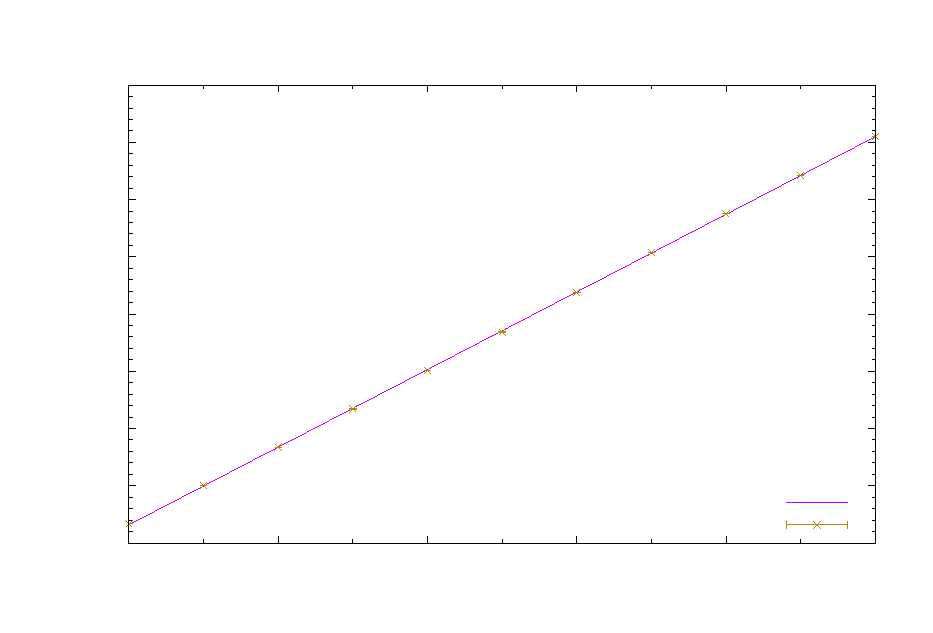
\includegraphics{tv3-plot}}%
    \gplfronttext
  \end{picture}%
\endgroup

		\caption{\centering Messung der Oberschwingungen des Rohres\captionbr $\chi^2_{\text{red}} = \num{46.698} > 1 \implies$ Schlechte Anpassung}
		\label{fig:tvthree-plot}
		\vspace{-1em}
	\end{figure}
	Die schlechte Anpassung kann vermutlich dadurch erklärt werden, dass die Bestimmung der Resonanzfrequenzen eher ungenau war, besonders bei der Steuerung des Sinus-Generator. In diesem Fall wurden aber die Messungenauigkeit der Frequenzen schon bei der Kurvenanpassung berücksichtigt. Es könnte dann sein, dass wir diese Ungenauigkeit wesentlich unterschätzt haben. 

	Als Endergebnis erhalten wir:
	\begin{center}
		\begin{tabular}{l r r}
			\toprule
			Variable & Rohausgabe & Gerundet \\
			\midrule
			$a$ & \SI{339,0636(6516)}{\hertz} & \SI{339.1(7)}{\hertz} \\
			$b$ & \SI{159.227(3855)}{\hertz} & \SI{159(4)}{\hertz} \\
			\bottomrule
		\end{tabular}
	\end{center}
	Wir benutzen in unserer Rechnungen die genauere Werte von $a$ und $\Delta a$ bzw. $v$ und $\Delta v$. In diesem Fall wurde für die Bestimmung der akustischen Rohrlänge aufgrund des geringeren Fehler $a$ statt $b$ gewählt, obwohl beide Werte theoretisch funktionieren könnten. 

	Mit der folgenden Werten:
    \begin{center}
        \begin{tabular}{lrl}
            \toprule
            Variable & Wert & Bedeutung \\
            \midrule
            $a$ & \SI{339,0636(6516)}{\hertz} & Gefundene Steigung der Gerade \\
            $v$ & \SI{344,424(1694)}{\meter\per\second} & Gefundene Schallgeschwindigkeit \\
            \bottomrule
        \end{tabular}
    \end{center}
    lässt sich mittels Gleichungen \eqref{eqn:akustiklange} und \eqref{eqn:deltaakustiklange} die akustische Rohrlänge $L^{*}$ und deren Fehler $\Delta L^{*}$ bestimmen:
    \begin{align}
    	L^{*} &= \frac{\SI{344,424}{\meter\per\second}}{2\pbrace{\SI{339,0636}{\hertz}}} = \SI{0,507905}{\meter} \sigfig{6} \\
    	\Delta L^{*} &= \frac{\SI{344,424}{\meter\per\second}}{2\pbrace{\SI{339,0636}{\hertz}}} \sqrt{\pbrace{\frac{\SI{1.694}{\meter\per\second}}{\SI{344,424}{\meter\per\second}}}^2 + \pbrace{\frac{\SI{0.6516}{\hertz}}{\SI{339,0636}{\hertz}}}^2} \notag \\
    	&= \SI{2,682e-3}{\meter} \sigfig{4}
    \end{align}
    Daraus folgt, dass die akustische Rohrlänge $L^{*} = \SI{0,5079(27)}{\meter} = \SI{507.9(27)}{\milli\meter}$.

    Im Vergleich dazu ist die gemessene Rohrlänge $L = \SI{50.0(1)}{\centi\meter} = \SI{500(1)}{\milli\meter}$. Das Fehlerintervall der beiden Werten überschneiden sich miteinander nicht, also ist $L^{*} > L$, was zu erwarten ist. 
\newpage
\section{Teilversuch 4: Messung der Resonanzkurve für eine Oberschwingung}
	\subsection{Messreihe}
	Fehler der Frequenzen $\Delta f = \SI{1}{\hertz}$ \\
	Fehler der Spannung $\Delta f = \SI{0.2}{\milli\volt}$

	Raumhintergrund $= \SI{1.1(2)}{\milli\volt}$

	\begin{center}
		\begin{tabular}{l *{10}{r}}
			\toprule
			$f / \si{\hertz}$ & \num{1011} & \num{980} & \num{970} & \num{952} & \num{928} & \num{910} & \num{892} & \num{881} & \num{871} & \num{861} \\
			\midrule
			$U_\text{eff} / \si{\milli\volt}$ & \num{7.33} & \num{7.53} & \num{7.99} & \num{8.85} & \num{10.85} & \num{13.45} & \num{18.33} & \num{23.31} & \num{30.14} & \num{44.53} \\
			\bottomrule
			\toprule
			$f / \si{\hertz}$ & \num{854} & \num{850} & \num{844} & \num{841} & \num{837} & \num{833} & \num{830} & \num{825} & \num{818} & \num{810} \\
			\midrule
			$U_\text{eff} / \si{\milli\volt}$ & \num{64.33} & \num{85.80} & \num{125.53} & \num{149.11} & \num{149.49} & \num{120.65} & \num{96.04} & \num{71.73} & \num{54.43} & \num{41.24} \\
			\bottomrule
			\toprule
			$f / \si{\hertz}$ & \num{801} & \num{790} & \num{780} & \num{760} & \num{742}  \\
			\midrule
			$U_\text{eff} / \si{\milli\volt}$ & \num{34.00} & \num{28.51} & \num{25.66} & \num{22.68} & \num{21.61} \\
			\bottomrule
		\end{tabular}
	\end{center}

	\subsection{Graph}
	Aus der Anleitung des Versuchs MOS lässt die folgende Funktion eine Resonanzkurve beschreiben:
	\begin{equation}
		\hat{x} = \frac{\omega_0^2}{\sqrt{\pbrace{\omega_0^2 - \omega^2}^2+\pbrace{2\beta\omega}^2}}~\hat{x}_\text{A} \iff U_\text{eff} = \frac{f_0^2}{\sqrt{\pbrace{f_0^2 - f^2}^2+\pbrace{2\beta f}^2}}~U_\text{A}
	\end{equation}

	Da die Kurvenanpassung mit \gnuplot{} sehr empfindlich auf die Wahl der Startparameter reagiert, müssen die Startparameter sorgfältig ausgewählt. Dafür ist eine grobe Kurveanpassung wie im Versuch MOS mittels Geogebra per Hand durchgeführt:
	\begin{figure}[H]
		\centering
		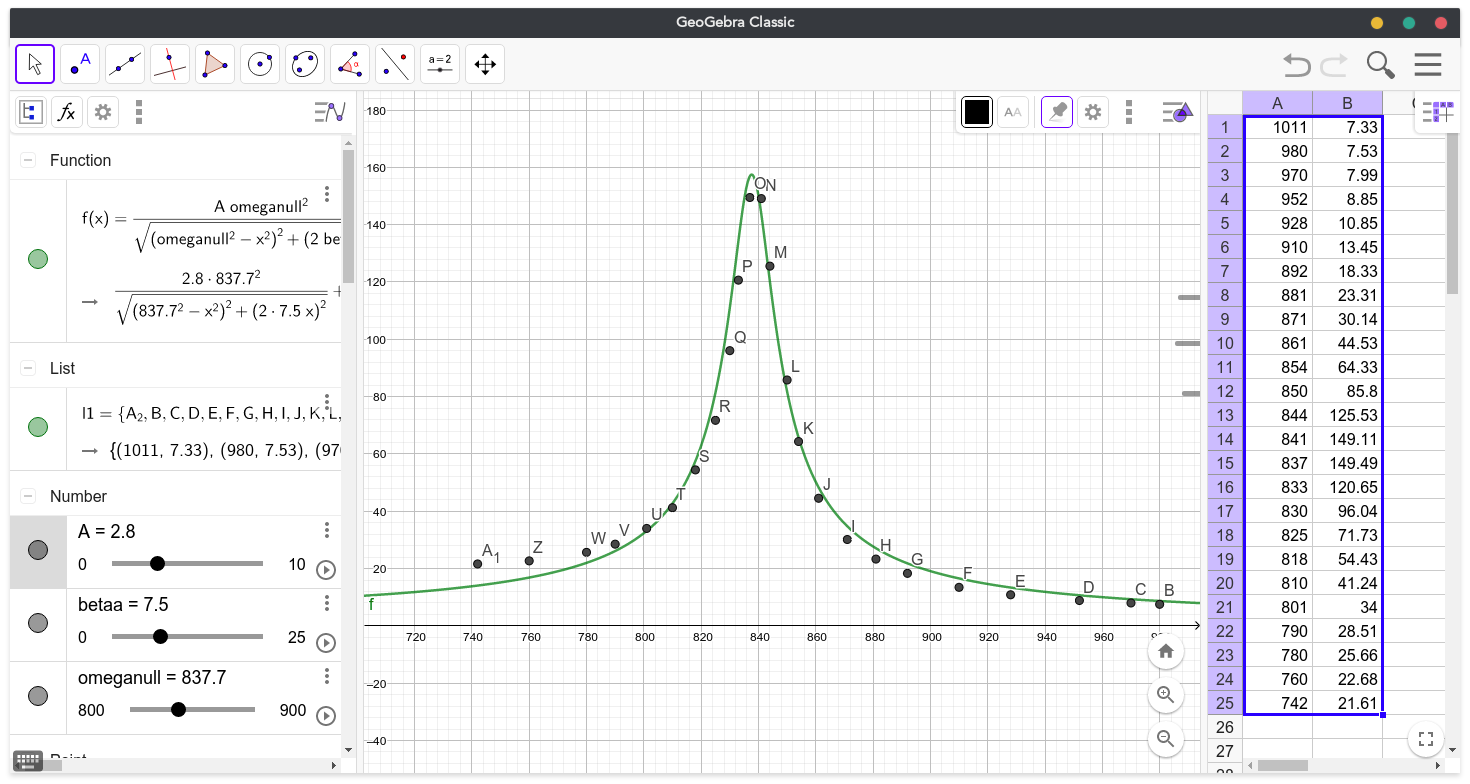
\includegraphics[width=0.9\textwidth]{geogebra.png}
		\caption{Grobe Kurveanpassung mittels Geogebra}
	\end{figure}

	Der Raumhintergrund und dessen Fehler sind direkt im \gnuplot{} Skript berücksichtigt (Siehe Appendix \ref{appdx:gnuplotTV4}). Der Fehler der Spannung nach dem Abzug des Raumhintergrund wird als $(\SI{0.2}{\milli\volt} + \SI{0.2}{\milli\volt} = \SI{0.4}{\milli\volt})$ angenommen. Der Grund dafür ist, dass wir letztendlich nur eine Messung von der Raumhintergrund haben, obwohl wir bei mehrfache Messungen eher Schwankungen gegen die gleiche Werten bekommen. Daher ist es sicherer bei der Kurvenanpassung einen größeren Fehler zu benutzen.

	\begin{figure}[H]
		\centering
		% GNUPLOT: LaTeX picture with Postscript
\begingroup
  \makeatletter
  \providecommand\color[2][]{%
    \GenericError{(gnuplot) \space\space\space\@spaces}{%
      Package color not loaded in conjunction with
      terminal option `colourtext'%
    }{See the gnuplot documentation for explanation.%
    }{Either use 'blacktext' in gnuplot or load the package
      color.sty in LaTeX.}%
    \renewcommand\color[2][]{}%
  }%
  \providecommand\includegraphics[2][]{%
    \GenericError{(gnuplot) \space\space\space\@spaces}{%
      Package graphicx or graphics not loaded%
    }{See the gnuplot documentation for explanation.%
    }{The gnuplot epslatex terminal needs graphicx.sty or graphics.sty.}%
    \renewcommand\includegraphics[2][]{}%
  }%
  \providecommand\rotatebox[2]{#2}%
  \@ifundefined{ifGPcolor}{%
    \newif\ifGPcolor
    \GPcolortrue
  }{}%
  \@ifundefined{ifGPblacktext}{%
    \newif\ifGPblacktext
    \GPblacktexttrue
  }{}%
  % define a \g@addto@macro without @ in the name:
  \let\gplgaddtomacro\g@addto@macro
  % define empty templates for all commands taking text:
  \gdef\gplbacktext{}%
  \gdef\gplfronttext{}%
  \makeatother
  \ifGPblacktext
    % no textcolor at all
    \def\colorrgb#1{}%
    \def\colorgray#1{}%
  \else
    % gray or color?
    \ifGPcolor
      \def\colorrgb#1{\color[rgb]{#1}}%
      \def\colorgray#1{\color[gray]{#1}}%
      \expandafter\def\csname LTw\endcsname{\color{white}}%
      \expandafter\def\csname LTb\endcsname{\color{black}}%
      \expandafter\def\csname LTa\endcsname{\color{black}}%
      \expandafter\def\csname LT0\endcsname{\color[rgb]{1,0,0}}%
      \expandafter\def\csname LT1\endcsname{\color[rgb]{0,1,0}}%
      \expandafter\def\csname LT2\endcsname{\color[rgb]{0,0,1}}%
      \expandafter\def\csname LT3\endcsname{\color[rgb]{1,0,1}}%
      \expandafter\def\csname LT4\endcsname{\color[rgb]{0,1,1}}%
      \expandafter\def\csname LT5\endcsname{\color[rgb]{1,1,0}}%
      \expandafter\def\csname LT6\endcsname{\color[rgb]{0,0,0}}%
      \expandafter\def\csname LT7\endcsname{\color[rgb]{1,0.3,0}}%
      \expandafter\def\csname LT8\endcsname{\color[rgb]{0.5,0.5,0.5}}%
    \else
      % gray
      \def\colorrgb#1{\color{black}}%
      \def\colorgray#1{\color[gray]{#1}}%
      \expandafter\def\csname LTw\endcsname{\color{white}}%
      \expandafter\def\csname LTb\endcsname{\color{black}}%
      \expandafter\def\csname LTa\endcsname{\color{black}}%
      \expandafter\def\csname LT0\endcsname{\color{black}}%
      \expandafter\def\csname LT1\endcsname{\color{black}}%
      \expandafter\def\csname LT2\endcsname{\color{black}}%
      \expandafter\def\csname LT3\endcsname{\color{black}}%
      \expandafter\def\csname LT4\endcsname{\color{black}}%
      \expandafter\def\csname LT5\endcsname{\color{black}}%
      \expandafter\def\csname LT6\endcsname{\color{black}}%
      \expandafter\def\csname LT7\endcsname{\color{black}}%
      \expandafter\def\csname LT8\endcsname{\color{black}}%
    \fi
  \fi
    \setlength{\unitlength}{0.0500bp}%
    \ifx\gptboxheight\undefined%
      \newlength{\gptboxheight}%
      \newlength{\gptboxwidth}%
      \newsavebox{\gptboxtext}%
    \fi%
    \setlength{\fboxrule}{0.5pt}%
    \setlength{\fboxsep}{1pt}%
\begin{picture}(8640.00,5760.00)%
    \gplgaddtomacro\gplbacktext{%
      \csname LTb\endcsname%%
      \put(814,704){\makebox(0,0)[r]{\strut{}$0$}}%
      \put(814,1253){\makebox(0,0)[r]{\strut{}$20$}}%
      \put(814,1803){\makebox(0,0)[r]{\strut{}$40$}}%
      \put(814,2352){\makebox(0,0)[r]{\strut{}$60$}}%
      \put(814,2902){\makebox(0,0)[r]{\strut{}$80$}}%
      \put(814,3451){\makebox(0,0)[r]{\strut{}$100$}}%
      \put(814,4000){\makebox(0,0)[r]{\strut{}$120$}}%
      \put(814,4550){\makebox(0,0)[r]{\strut{}$140$}}%
      \put(814,5099){\makebox(0,0)[r]{\strut{}$160$}}%
      \put(946,484){\makebox(0,0){\strut{}$700$}}%
      \put(1988,484){\makebox(0,0){\strut{}$750$}}%
      \put(3031,484){\makebox(0,0){\strut{}$800$}}%
      \put(4073,484){\makebox(0,0){\strut{}$850$}}%
      \put(5116,484){\makebox(0,0){\strut{}$900$}}%
      \put(6158,484){\makebox(0,0){\strut{}$950$}}%
      \put(7201,484){\makebox(0,0){\strut{}$1000$}}%
      \put(8243,484){\makebox(0,0){\strut{}$1050$}}%
    }%
    \gplgaddtomacro\gplfronttext{%
      \csname LTb\endcsname%%
      \put(209,2901){\rotatebox{-270}{\makebox(0,0){\strut{}Mikrofonspannung $U_\text{eff}$ ($\si{\milli\volt}$)}}}%
      \put(4594,154){\makebox(0,0){\strut{}Frequenz $f$ ($\si{\hertz}$)}}%
      \put(4594,5429){\makebox(0,0){\strut{}Resonanzkurve des Rohres bei der 2. Oberschwingung}}%
      \csname LTb\endcsname%%
      \put(7256,4926){\makebox(0,0)[r]{\strut{}Angepasste Kurve}}%
      \csname LTb\endcsname%%
      \put(7256,4706){\makebox(0,0)[r]{\strut{}Messpunkte}}%
    }%
    \gplbacktext
    \put(0,0){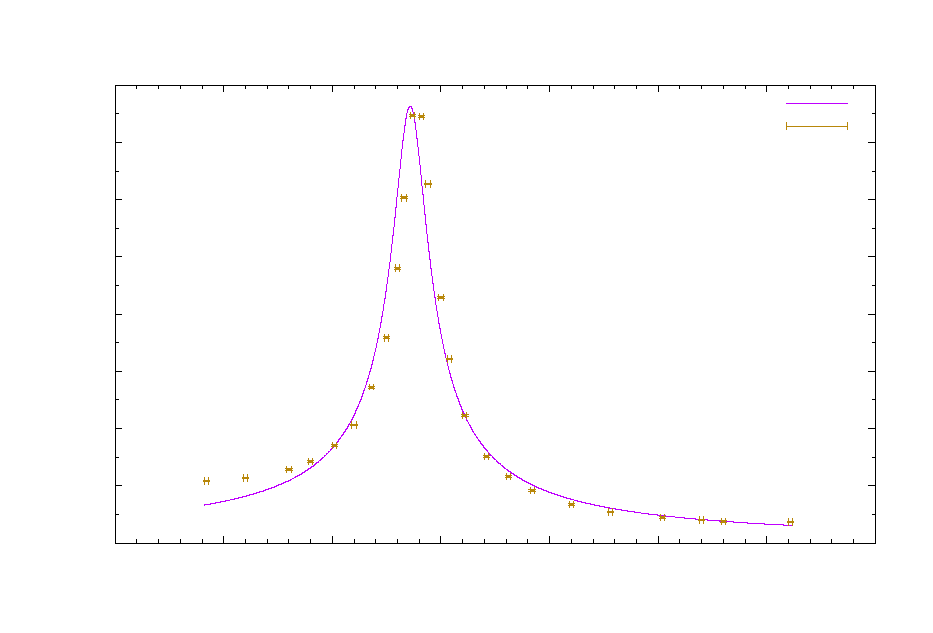
\includegraphics{tv4-plot}}%
    \gplfronttext
  \end{picture}%
\endgroup

		\caption{\centering Messung der Resonanzkurve des Rohres bei der 2. Oberschwingung\captionbr $\chi^2_{\text{red}} = \num{32.6373} > 1 \implies$ Schlechte Anpassung}
		\label{fig:tvfour-plot}
		\vspace{-1em}
	\end{figure}
	Als Endergebnis erhalten wir:
	\begin{center}
		\begin{tabular}{l r r}
			\toprule
			Variable & Rohausgabe & Gerundet \\
			\midrule
			$f_0$ & \SI{835.89(146)}{\hertz} & \SI{835.9(15)}{\hertz} \\
			$U_\text{A}$ & \SI{2.8473(1317)}{\milli\volt} & \SI{2.85(14)}{\milli\volt} \\
			$\beta$ & \num{7.79(102)} & \num{7.8(11)} \\
			\bottomrule
		\end{tabular}
	\end{center}

	Anstatt einfach die Messpunkte durch eine glatte Kurve zu verbinden, war eine theoretische Kurve auf die Messwerte angepasst. Die Anpassung war leider schlecht, und der Grund dafür liegt vermütlich daran, dass wir Nebeneffekte bzw. andere Faktoren nicht berücksichtigt haben. Es könnte auch sein, dass wir alle Werten im SI Einheiten skalieren sollten, bevor wir die Kurvenanpassung durchführen. 

	Unsere gemessene Resonanzfrequenz $f_0 = \SI{837(1)}{\hertz}$ liegt auch im Fehlerintervall des aus der Kurvenanpassung gefundene $f_0$. Die Werte stimmen also miteinander überein.

\resnum
\newpage
\appendix
\section{\gnuplot{} Quellcode zur Auswertung von Teilversuch 1}
	\label{appdx:gnuplotTV1}

	\gnuplot{} Code für Abbildung \ref{fig:tvone-plot}
	{  
        % % Surpress "errors" in minted
        % https://tex.stackexchange.com/a/289068
        \renewcommand{\fcolorbox}[4][]{#4}
        \begin{minted}[linenos,breaklines,autogobble,frame=leftline,framesep=10pt]{gnuplot}
#!/usr/bin/env gnuplot
# ver >= 5.2

set term epslatex color size 6in, 4in
set output "tv1-plot.tex"
set decimalsign locale 'de_DE.UTF-8'

set title "Mikrofonspannung als Funktion der Position"
set xlabel "Position auf optischen Schiene $x$ ($\\si{\\milli\\meter}$)"
set ylabel "Mikrofonspannung $U_\\text{eff}$ ($\\si{\\milli\\volt}$)"

set mxtics
set mytics
set samples 10000

A = 45
b = 95.2
lambda = 134.75
c = 2
f(x) = abs(A*sin(((2*pi)/lambda)*(x - b))) + c

# (x, y, xdelta, ydelta)
fit f(x) "tv1.dat" u 1:2:(0.5):3 xyerrors via A,lambda,b,c

# Anomalie
set style fill solid 0.0 border 7
set object circle at 87.5, 25 size 2 fc rgb 'black'
set label "\\textcolor{red}{\\scriptsize Anomalie}" at 85,27 font ',9'

# Linien
array oneleft[5]   = [93.5, 98.5, 89, 104.5, 87.5]
array oneright[5]  = [97, 89.5, 102, 84.5, 107]
array lastleft[5]  = [232, 225.5, 237.522, 220, 242]
array lastright[5] = [228, 234.5, 223, 237.5, 217.5]
set style fill solid 1.0 border -1
do for [i=1:5] {
    why = i*5
    onemw  = (oneleft[i] + oneright[i])/2
    lastmw = (lastleft[i] + lastright[i])/2

    #(x, y)
    set arrow from oneleft[i],why to oneright[i],why nohead lc rgb 'dark-green' # dt 3
    set arrow from lastleft[i],why to lastright[i],why nohead lc rgb 'dark-green' # dt 3

    set object circle at onemw,why size 0.4 fc rgb 'black'
    set object circle at lastmw,why size 0.4 fc rgb 'black'
}

set arrow from b,0 to b,25 nohead lc rgb 'orange'
set arrow from b+lambda,0 to b+lambda,25 nohead lc rgb 'orange'

set yrange [0:56]
set key top right spacing 1.8

titel = "$\\abs{".gprintf("%.5f", A)."\\sin\\left[\\frac{2\\pi}{".gprintf("%.5f", lambda)."}\\left(x - ".gprintf("%.5f", b)."\\right)\\right]} + ".gprintf("%.5f", c)."$"
plot f(x) title titel lc rgb 'dark-magenta', \
    "tv1.dat" u 1:2:(0.5):3 with xyerrorbars title "Messpunkte" pointtype 0 lc rgb 'dark-goldenrod', \
    "<echo 87,5 25,0" u 1:2:(0.5):(0.2) with xyerrorbars notitle pointtype 0 lc rgb 'red'
        \end{minted}
    }
    mit \texttt{tv1.dat}:
    \begin{multicols}{3}
        \begin{minted}[linenos,breaklines,autogobble,frame=leftline,framesep=10pt]{text}
# x/mm  U/mV    delU
63,5    42,9    0,1
70,0    40,3    0,1
80,0    27,9    0,1
90,0    9,4     0,1
100,0   12,8    0,1
110,0   31,0    0,1
120,0   42,2    0,1
130,0   45,1    0,1
140,0   39,7    0,1
150,0   26,2    0,1
160,0   7,0     0,1
170,0   15,5    0,1
180,0   33,2    0,1
190,0   42,6    0,1
200,0   44,1    0,1
210,0   36,4    0,1
220,0   21,0    0,1
230,0   2,0     0,1
240,0   20,7    0,1
250,0   36,3    0,1
260,0   44,2    0,1
270,0   43,1    0,1
280,0   33,3    0,1
93,5    5,0     0,2
98,5    10,0    0,2
89,0    15,0    0,2
104,5   20,0    0,2
# 87,5  25,0    0,2
97,0    5,0     0,2
89,5    10,0    0,2
102,0   15,0    0,2
84,5    20,0    0,2
107,0   25,0    0,2
232,0   5,0     0,2
225,5   10,0    0,2
237,5   15,0    0,2
220,0   20,0    0,2
242,0   25,0    0,2
228,0   5,0     0,2
234,5   10,0    0,2
223,0   15,0    0,2
237,5   20,0    0,2
217,5   25,0    0,2
        \end{minted}
    \end{multicols}
    \vspace{-\baselineskip}
    Rohausgabe
    \begin{minted}[linenos,breaklines,autogobble,frame=leftline,framesep=10pt]{text}
degrees of freedom    (FIT_NDF)                        : 38
rms of residuals      (FIT_STDFIT) = sqrt(WSSR/ndf)    : 1.93411
variance of residuals (reduced chisquare) = WSSR/ndf   : 3.7408
p-value of the Chisq distribution (FIT_P)              : 6.03961e-14

Final set of parameters            Asymptotic Standard Error
=======================            ==========================
A               = 43.0608          +/- 0.5247       (1.219%)
lambda          = 135.638          +/- 0.3153       (0.2324%)
b               = 94.4062          +/- 0.2371       (0.2511%)
c               = 1.62297          +/- 0.4747       (29.25%)
    \end{minted}
\newpage
\section{\texttt{python} Quellcode zur Berechnung der Mittelwert und Standardabweichung im Teilversuch 1}
    \label{appdx:pythontv1}
    \begin{minted}[linenos,breaklines,autogobble,frame=leftline,framesep=10pt]{python}
#!/usr/bin/env python3

import numpy as np

x12 = np.array([95.25, 94.00, 95.50, 94.50])
x34 = np.array([230.00, 230.00, 230.26, 228.75, 229.75])

def sab(arr, mw):
    return np.sqrt((np.sum((arr - mw)**2))/(arr.size - 1))

x12mw = np.mean(x12)
x12ab = sab(x12, x12mw)
x34mw = np.mean(x34)
x34ab = sab(x34, x34mw)

print("x12 = ", x12mw, " +- ", x12ab)
print("x34 = ", x34mw, " +- ", x34ab)
    \end{minted}
    Rohausgabe
    \begin{minted}[linenos,breaklines,autogobble,frame=leftline,framesep=10pt]{python}
x12 =  94.8125  +-  0.688446318411
x34 =  229.752  +-  0.588447108923
    \end{minted}

\section{\gnuplot{} Quellcode zur Auswertung von Teilversuch 3}
    \label{appdx:gnuplotTV3}
    \gnuplot{} Code für Abbildung \ref{fig:tvthree-plot}
    {  
        % % Surpress "errors" in minted
        % https://tex.stackexchange.com/a/289068
        \renewcommand{\fcolorbox}[4][]{#4}
        \begin{minted}[linenos,breaklines,autogobble,frame=leftline,framesep=10pt]{gnuplot}
#!/usr/bin/env gnuplot

set term epslatex color size 6in, 4in
set output "tv3-plot.tex"
set decimalsign locale 'de_DE.UTF-8'

set title "Oberschwingungen"
set xlabel "Ordnungszahl $n$"
set ylabel "Frequenz $f_n$ ($\\si{\\hertz}$)"

set mxtics
set mytics

set key right bottom

f(x) = m*x + c

# (x, y, xdelta, ydelta)
fit f(x) "tv3.dat" u 1:2:(1) yerrors via m,c

titel = gprintf("%.6f", m)."n + ".gprintf("%.6f", c)
plot f(x) title titel lc rgb 'dark-magenta', \
    "tv3.dat" u 1:2:(1) with yerrorbars title "Messpunkte" lc rgb 'dark-goldenrod'
        \end{minted}
    }
    mit \texttt{tv3.dat}:
    \begin{minted}[linenos,breaklines,autogobble,frame=leftline,framesep=10pt]{text}
# n f/Hz    Ueff/mV
0   168     3,36
1   502     22,10
2   837     57,70
3   1171    31,07
4   1510    21,70
5   1843    22,48
6   2188    22,93
7   2541    24,80
8   2876    13,20
9   3210    10,10
10  3554    6,76
    \end{minted}
    Rohausgabe
    \begin{minted}[linenos,breaklines,autogobble,frame=leftline,framesep=10pt]{text}
degrees of freedom    (FIT_NDF)                        : 9
rms of residuals      (FIT_STDFIT) = sqrt(WSSR/ndf)    : 6.83359
variance of residuals (reduced chisquare) = WSSR/ndf   : 46.698
p-value of the Chisq distribution (FIT_P)              : 0

Final set of parameters            Asymptotic Standard Error
=======================            ==========================
m               = 339.064          +/- 0.6516       (0.1922%)
c               = 159.227          +/- 3.855        (2.421%)

correlation matrix of the fit parameters:
                m      c      
m               1.000 
c              -0.845  1.000
    \end{minted}

\section{\gnuplot{} Quellcode zur Auswertung von Teilversuch 4}
    \label{appdx:gnuplotTV4}

    \gnuplot{} Code für Abbildung \ref{fig:tvfour-plot}
    {  
        % % Surpress "errors" in minted
        % https://tex.stackexchange.com/a/289068
        \renewcommand{\fcolorbox}[4][]{#4}
        \begin{minted}[linenos,breaklines,autogobble,frame=leftline,framesep=10pt]{gnuplot}
#!/usr/bin/env gnuplot

set term epslatex color size 6in, 4in
set output "tv4-plot.tex"
set decimalsign locale 'de_DE.UTF-8'

set title "Resonanzkurve des Rohres bei der 2. Oberschwingung"
set xlabel "Frequenz $f$ ($\\si{\\hertz}$)"
set ylabel "Mikrofonspannung $U_\\text{eff}$ ($\\si{\\milli\\volt}$)"

set mxtics
set mytics
set samples 10000

omeganull = 837.7
beta = 7.4
A = 3
f(x) = (A*omeganull**2)/(sqrt((omeganull**2 - x**2)**2 + (2*beta*x)**2))

# (x, y, xdelta, ydelta)
fit f(x) "tv4.dat" u 1:($2-1.1):(1):(2*0.2) xyerrors via omeganull,beta,A

titel = "Angepasste Kurve"
plot f(x) title titel lc rgb 'dark-magenta', \
    "tv4.dat" u 1:2:(1):(sqrt(2)*0.2) with xyerrorbars title "Messpunkte" pointtype 0 lc rgb 'dark-goldenrod'
        \end{minted}
    }
    mit \texttt{tv4.dat}:
    \begin{multicols}{3}
        \begin{minted}[linenos,breaklines,autogobble,frame=leftline,framesep=10pt]{text}
#f/Hz   Ueff/mV
1011    7,33
980     7,53
970     7,99
952     8,85
928     10,85
910     13,45
892     18,33
881     23,31
871     30,14
861     44,53
854     64,33
850     85,80
844     125,53
841     149,11
837     149,49
833     120,65
830     96,04
825     71,73
818     54,43
810     41,24
801     34,00
790     28,51
780     25,66
760     22,68
742     21,61
        \end{minted}
    \end{multicols}
    \vspace{-\baselineskip}
    Rohausgabe
    \begin{minted}[linenos,breaklines,autogobble,frame=leftline,framesep=10pt]{text}
degrees of freedom    (FIT_NDF)                        : 22
rms of residuals      (FIT_STDFIT) = sqrt(WSSR/ndf)    : 5.71291
variance of residuals (reduced chisquare) = WSSR/ndf   : 32.6373
p-value of the Chisq distribution (FIT_P)              : 0

Final set of parameters            Asymptotic Standard Error
=======================            ==========================
omeganull       = 835.893          +/- 1.46         (0.1746%)
beta            = 7.79227          +/- 1.02         (13.09%)
A               = 2.8473           +/- 0.1317       (4.626%)
    \end{minted}

\end{document}
